Computer hardware has had an amazing increase on performance for decades, though for natively parallel problems these increases have not been enough. Special hardware emerged to solve specific tasks like video decoding or computer graphics, and general purpose processors adopted a multi-core design to alleviate performance needs. For neural-like computations, there has been an increase in custom hardware platforms which will be reviewed in this chapter.

\section{Classical computing}
Classical Von-Neumann computing has brought modern day wonders like personal computers that ease the tasks like writing a novel, calculating incomes and expenses, watching films or talking to relatives living far away. 

As central processing units (CPUs) achieve higher clock frequencies their power consumption increases as well. This is commonly mitigated because newer generations are usually manufactured using smaller transistors, and since they need less power to operate the whole processor consumes less energy. The technology to manufacture such machines is now reaching physical limits and performance is not increasing as expected. One solution to this is to pack multiple processing cores in a single computing unit and run tasks in parallel, which has alleviated the performance hunger for the time being (Figure~\ref{fig:comp:moore}). 

\begin{figure}[h]
  \begin{center}
    \includegraphics[width=0.7\textwidth]{integer-perf}%performance_growth
    \caption{Performance of CPUs vs release year, a steady increase is observed until about 2004, after that computing platforms where almost forced to use parallel processing~\cite{int-perf-images}. }%\cite{mips-perf-image}
    \label{fig:comp:moore}
  \end{center}
\end{figure}

Even though classic CPUs have tremendous computing power, they have not been able to perform well on tasks that humans do without noticing (e.g. pattern recognition, inference, puzzles). This has lead computer manufacturers to design specialized processors to increase performance for specific tasks. A particularly successful example of this are 3D graphics accelerating cards, also known as Graphic Processing Units (GPUs), that began life accelerating the transformation of 3D primitives onto 2D screens. More recently, the multiple parallel computation units that enable this, have become powerful and flexible enough to allow these devices to be used for general purpose computation.
%They use multiple parallel processing units to calculate, which are a great match to the parallel nature of graphics computations~\cite{nickolls2010gpu,chen2009gpu}. Lately, general processing has been made possible in these cards though commercial applications other than graphics are just starting to emerge. 
Although GPUs are now considered highly parallel computing platforms and could be seen as a natural fit for neural networks, the data communication strategies are of a different nature and GPUs consume large amounts of power (high performance cards are rated at $>$ 300 watts)~\cite{nvidia, amd}.



\section{Neuromorphic trends}
Artificial intelligence (AI) is another field of computing which strains classical computers, so building systems that can achieve anything resembling intelligence requires very powerful computers. In 1997, IBM's Deep Blue computer won a game of chess to human master Garry Kasparov, relying on 480 specialized chess chips that performed massively parallel game moves searches~\cite{deep-blue-Campbell200257}. Although it was not the first attempt at hardware-based AI~\cite{indiveri2011frontiers}, it was probably the first time a general audience got to know that a computer could beat a human being on cognitive tasks. 

This great achievement may be dwarfed by the fact that humans can do much more than play chess and Deep Blue was nowhere near ready to do the laundry or pick up the kids from school. A general solution is still the holly grail of AI and, as research on the brain advances, scientists have taken inspiration from biology to develop new computing platforms. 
%Researchers have built custom hardware to solve AI problems as early as 1958~\cite{indiveri2011frontiers}. 
The term \emph{neuromorphic} (i.e. that resembles neural form) is attributed to \citeauthor{mead2012analog}, probably coined as he worked on the implementation of silicon retinas~\cite{carver-mead,mead2012analog}. The main advantages of hardware that lies on the neuromorphic range are, low power consumption, real-time functionality, scalability and fault tolerance. More work has been done on neuromorphic sensors that have lead to silicon retinas, cochleas or visual motion sensors, to name a few~\cite{liu2010neuromorphic}. While sensory input is of utmost importance for every system, a platform to make use of these sensors for AI tasks is still an open research problem. 

Hardware platforms that combine the knowledge acquired from neuroscience and artificial neural networks research have been recently developed. They may be classified based on the type of hardware/software combination used. Hardware neurons are analog circuits that behave like a mathematical model of a neuron; software neurons simulate the model using a general digital processor. Similar distinctions can be made for synapses, axonal and dendritic trees~\cite{misra2010artificial}. There are several projects implementing hardware neural platforms, the following are the most important ones~\cite{neuro-platforms-summary-7159144}.

The \emph{BrainScales} project is carried by multiple universities and research institutes - based on FACETS, exponential integrate and fire, short term depression and facilitation, stdp, programmable topology and parameters

\emph{Neurogrid} - custom model, hardware model, ram weights converted with Digital to Analog Converters (DACs), digital network for spikes

\emph{TrueNorth} - event driven, software neurons, binary programmable synapses, 
\section{SpiNNaker}
The \textbf{SpiNNaker} system is a massively-parallel, bio-inspired computing platform. The goal of the project is to build a machine that will contain $\sim$1 million CPU cores and will be able to simulate $\sim$1 billion neurons in real time. As any multi-core system, communication between cores is basic; the SpiNNaker chip has been designed to efficiently implement neural networks, thus, networking is specialized (but not limited) to transmit spikes. There are currently two board models the Spinn-3, which hosts 4 SpiNNaker chips, and the Spinn-4 that houses 48 nodes. These boards are also known as 102 and 103 machines, respectively. Larger systems will be built using Spinn-4 boards as the basic construction block. Plans include building the following: 
\begin{description}
  \item[104 machine], a 12 Spinn-4 desktop frame with $\sim$10000 ARM cores.
  \item[105 machine], five card frames with 24 Spinn-4 each allocated in a rack cabinet ($\sim$100,000 cores).
  \item[106 machine], 10 racks, each with similar capacities of the 105 machine ($\sim$1,000,000 cores).
\end{description}

\subsection{SpiNNaker chip overview}

SpiNNaker chips consist of 18 ARM968 cores, each with tightly-coupled program and data memory. Each core also has a Communication Network-on-Chip (C-NoC) interface that, with the help of an in-die network router, allows inter- and intra-chip communications (Figure~\ref{fig:hw:spinnaker-die}). On top of the chip lie 128 MBytes of Synchronous Dynamic RAM (SDRAM) whose die is stitch-bonded to the chip for faster access (Figure~\ref{fig:hw:bonded-sdram}). The SpiNNaker chip plus the SDRAM are sometimes referred as a \emph{node}~\cite{furber2013overview}.

\begin{figure}[h]
  \begin{center}
    \begin{subfigure}[b]{0.55\textwidth}
      \includegraphics[width=\textwidth]{spinn_labeled_bw}
      \caption{SpiNNaker chip die.}
      \label{fig:hw:spinnaker-die}
    \end{subfigure}
    \hspace*{0.3cm}
    \begin{subfigure}[b]{0.4\textwidth}
      \includegraphics[width=\textwidth]{spinn_dies-ram}
      \caption{Stitch-bonded SDRAM on top of the SpiNNaker chip.}
      \label{fig:hw:bonded-sdram}
    \end{subfigure}
    \caption{SpiNNaker base component, a node, consists of a multi-core chip with stitch-bonded SDRAM.}
  \end{center}
\end{figure}

One of the cores acts as a system controller and, typically, 16 cores will run the applications. Any processor in a chip will have access to four memory spaces. Instruction and data memories are only locally visible (i.e. a core can only see its local memory). These two spaces are composed of a 32 and 64 KByte tightly-coupled blocks of memory, respectively. There are also a 32 KByte block of on-chip SRAM and the 128 MByte off-die SDRAM, both of them are node-local (i.e. seen by all processors in the chip). The cores are able to access the SDRAM and SRAM using the System Network-on-Chip (S-NoC) and no inter-chip memory coherence mechanisms are present~\cite{furber2013overview}. SDRAM is commonly used for large data structures like synaptic weight matrices, while the SRAM is used for core-to-core message passing.

\subsection{Communications}

One of the notable aspects of the SpiNNaker system is the flexibility of its networking infrastructure. Communication in the global scale is asynchronous and locally synchronous. There are six direct links from any source node to its neighbours. This provides sufficient connections to form an efficient network that may be configured to form a toroid (Figure~\ref{fig:hw:spinn-toroid}) on a 2D circuit board.

\begin{figure}[h]
  \begin{center}
    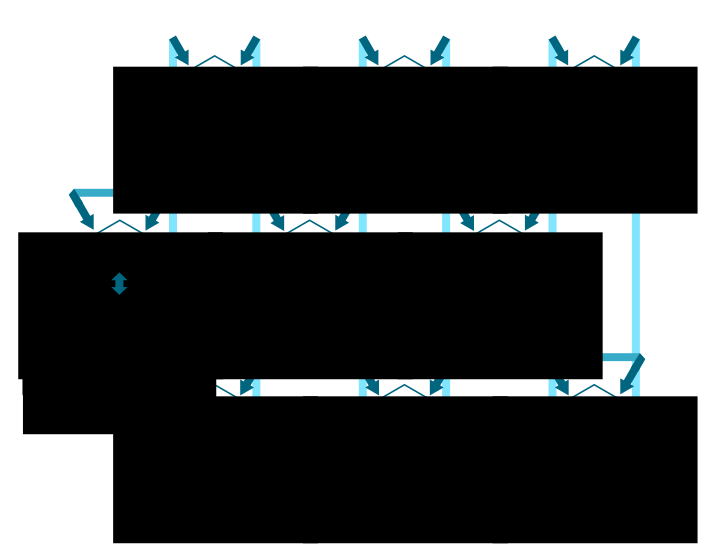
\includegraphics[width=0.7\textwidth]{spinn-interconect}
    \caption{Nine SpiNNaker nodes connected as a toroid.}
    \label{fig:hw:spinn-toroid}
  \end{center}
\end{figure}

Packets are the only way a SpiNNaker chip can communicate to another; a core sends a packet to the local router where it's forwarded to one or more targets. If the target is in the same node, the router will deliver it directly; otherwise, the router sends the packet to an adjacent node where the next router will decide the appropriate move. Packets are either 40 or 72 bit long, a control byte, and one or two 32-bit words.

There are four ways a packet types, each of which are routed differently by the router. \emph{Nearest neighbour} (NN) and \emph{point-to-point} (P2P) packets are may be generated by any core, but will only reach the monitor core on the target node. NN packets are mainly used for boot and recovery and P2P for code distribution and system control. \emph{Fixed route} (FR) packets may be emitted by any core and sent to any other core, though the route is may not be changed once an application is running. This packet type is generally used for debugging purposes.
The \emph{multicast} (MC) packet also permits core-to-core transmission, so applications use this type to transmit data. If the packet has multiple targets, a router along the way will duplicate it and fork the route. This is a highly desired feature for neural applications, since one neuron's axon may connect to multiple neurons dendrites~\cite{spinn-net-patterson2012scalable}. MC packets are formed using address event representation (AER), so they posses a time-stamp and a full source address (node, core, and neuron identifications).

Communication to the outside world is done through 100 Mbit/s Ethernet, General Purpose Input/Output (GPIO) lines and through Field-Programmable Gate Arrays (FPGAs, on the 48-node boards).

\subsection{Programming modes}
Since neurons are thought to react as spikes arrive at their dendrites, SpiNNaker chips support event-based usage via specialized interrupt hardware. There are, primarily, two choices while trying to program SpiNNaker. 

The first is through the application programming interface (API) following an event-driven model. In this way applications can only specify what functions to execute when an event occurred. Events include multicast packet reception, direct memory access (DMA) completion, timer ticks, SpiNNaker datagram protocol packet arrival, and custom user events. Using this type of programming allows developers to create not only neural network simulations but any application~\cite{spinn-software-docs}. 

The second is to use the neural network interface PyNN~\cite{davison2008pynn}, which provides a common front-end to different simulators (e.g. NEST, Brian, sPyNNaker). Since the descriptions are stated using the Python programming language and because it's a high level description, the learning curve for this approach is moderate~\cite{spynnaker-github}. A common PyNN application would set-up the simulator parameters, describe neural populations, establish the appropriate projections and start the simulation. The sPyNNaker team has added modules for real-time interaction with PyNN scripts and facilities for adding new neural and synaptic models.
%\section{Event-based model}
%\input{./chapters/neuromorphic_hardware/event_based}
\section{Conclusions}
Neuromorphic hardware presents advantages in terms of energy efficiency and can help to develop ``intelligent'' platforms that could perform human-like tasks (e.g. image recognition) without the need of a computer that requires a power plant to operate. Among large scale hardware based neural platforms, TrueNorth has a nice balance of programmability and power consumption but it's lack of synaptic plasticity and restricted networking make it less desirable. 
SpiNNaker's power consumption could be diminished if the chip manufacturing process was reduced from its current $130 nm$. The network fabric on SpiNNaker brings unprecedented flexibility and the fact that neurons, synapses and plasticity are programmable, make it an excellent choice for neuroscience research.